\documentclass[../main.tex]{subfiles}
\graphicspath{
    {"../img/"}
    {"img/"}
}

\begin{document}
    Rozważmy szereg
    \begin{equation}
        \label{eqn:fourierboy}
        \sum_{n=-\infty}^{\infty} c_n e^{2\pi i n x} \tag{$\mathcal{F}$}
    \end{equation}
gdzie
\[
    c_n = \int\limits_{-\frac{1}{2}}^{\frac{1}{2}} f(k) e^{-2\pi i n k}dk
.\]
Same nasuwają się pytania
\begin{enumerate}
    \item Czy ten szereg \eqref{eqn:fourierboy} jest zbieżny?
    \item Jak tak, to do czego?
\end{enumerate}

Pamiętamy twierdzenie
\begin{tw}
    Jeżeli $f\in\mathcal{C}^2\left(\left[-\frac{1}{2},\frac{1}{2}\right]\right)$, to
    \[
        \sum_{n=-\infty}^{\infty} \left| c_n e^{2\pi i n x} \right| \le \sum_{n=-\infty}^{\infty} \frac{1}{n^2}
    \]
    i szereg \eqref{eqn:fourierboy} zbiega do $f(x)$.
\end{tw}

Drugi wariant
\begin{tw}
    Jeżeli $f\in \mathcal{L}^2\left( \left[ -\frac{1}{2},\frac{1}{2} \right]  \right) $, to
    \[
        \sum_{n=-\infty}^{\infty} \left| c_n \right| ^2 \le \int\limits_{-\frac{1}{2}}^{\frac{1}{2}} \left| f(x) \right| ^2 dx
    ,\]
wówczas szereg po lewej jest zbieżny, czyli mamy jeszcze
\[
    \lim_{n \to \infty}c_n = 0
.\]
\end{tw}
\begin{pytanie}
    Jaka klasa funkcji nas interesuje?(\ref{fig:sygnal2}) (chcemy, żeby ładnie działało z \eqref{eqn:fourierboy}.
\end{pytanie}
\begin{figure}[h]
    \centering
    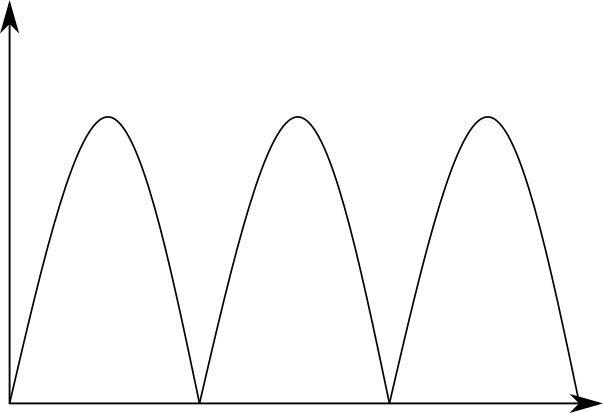
\includegraphics[width=0.4\textwidth]{sygnal1}
    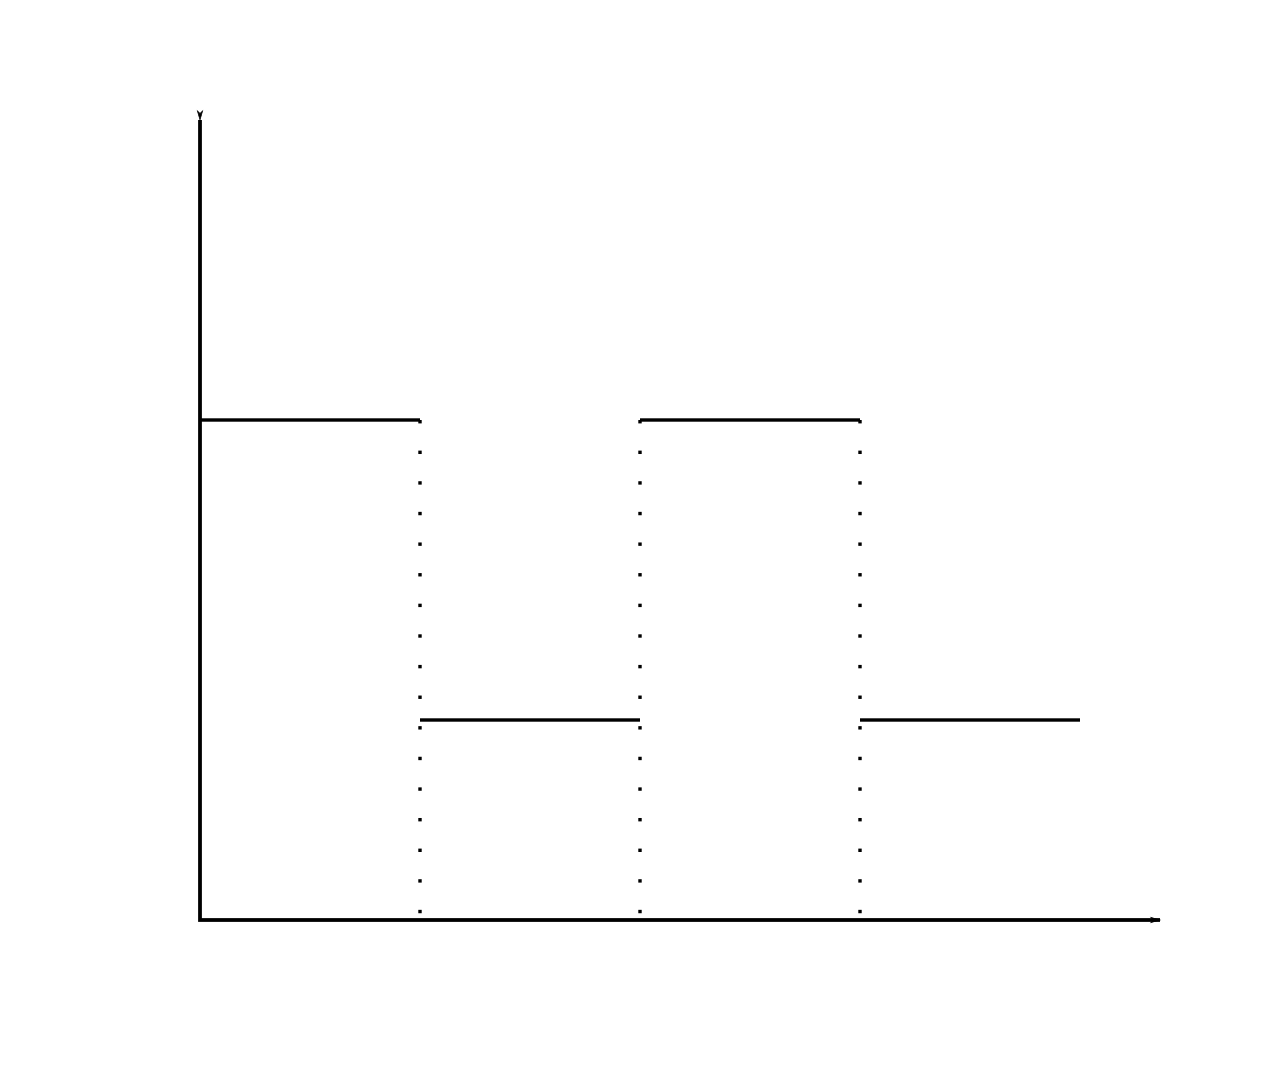
\includegraphics[width=0.4\textwidth]{sygnal2}
    \caption{Takie funkcje nam pasują na pewno}
    \label{fig:sygnal2}
\end{figure}
\begin{definicja}
    Mówimy, że $f(x)$ jest kawałkami ciągła na $\mathbb{R}$, jeżeli ma okres $1$, na przedziale $\left[ -\frac{1}{2},\frac{1}{2} \right] $ ma skończoną liczbę punktów nieciągłości.
\end{definicja}

\begin{tw}
    (Lemat 1)\\
    Niech
    \[
        D_N (\xi) = \sum_{n=-N}^{N} e^{-2\pi i n \xi}
    .\]
Wówczas
    \begin{enumerate}
    \item \[
            D_N(\xi) = \begin{cases}
                \frac{\sin\left( (N+\frac{1}{2}) \right) \frac{2\pi \xi}{2}}{\sin\left( \frac{2\pi \xi}{2} \right) } & \xi\in \left[ -\frac{1}{2},\frac{1}{2} \right]  \setminus \left\{ 0 \right\}\\
                2N + 1 & \xi = 0
            \end{cases}
    .\]
\item
    \[
        \int\limits_{-\frac{1}{2}}^{\frac{1}{2}} D_N(\xi) = 1 = 2 \int\limits_{0}^{\frac{1}{2}} D_N(\xi)
    .\]
\end{enumerate}
\end{tw}
\begin{proof}
    (część 2)\\
    \begin{align*}
        D_N(\xi) &= e^{2\pi i N \xi} + e^{2\pi i \xi (N - 1)} + \ldots + e^{2\pi i \xi} + 1 + e^{-2\pi i \xi} + \ldots =\\
        &= 1 + 2 \sum_{n=1}^{N} \cos(2\pi n \xi)
    .\end{align*}
    Wówczas
    \[
        \int\limits_{-\frac{1}{2}}^{\frac{1}{2}} D_N(\xi) = \int\limits_{-\frac{1}{2}}^{\frac{1}{2}} d\xi + 2 \sum_{n=1}^{N} \int\limits_{-\frac{1}{2}}^{\frac{1}{2}} \cos(2\pi n \xi)d\xi
    .\]
Każda taka całka jest równa $\left.\frac{1}{2\pi n}\sin(2\pi n \xi)\right|_{-\frac{1}{2}}^{\frac{1}{2}} = 0$
\end{proof}
\begin{proof}
    (część 1)\\
    Niech $2\pi \xi \equiv t$, wtedy nasze $D_N(\xi)$ jest takie.
    \begin{align*}
        D_N(\xi) &= e^{i t N} + e^{i t (N-1)} + \ldots + e^{it} + 1 + e^{-it} + \ldots + e^{-it(N-1)} + e^{-itN} = \\
        &= e^{-itN}(1 + e^{it} + \ldots + e^{2i tN}) = \\
        &= e^{-itN} \cdot \frac{1-e^{it(2N+1)}}{1-e^{it}} = \\
        &= \frac{e^{-itN}}{2i}\frac{2i \cdot 2i}{\left(-e^{\frac{it}{2}}\right)\left(e^{\frac{it}{2}} - e^{-\frac{it}{2}}\right)} \cdot \frac{\left(-e^{it\frac{2N+1}{2}}\right)\left(e^{it\frac{2N+1}{2}} - e^{-it\frac{2N+1}{2}}\right)}{2i} = \\
        &= \frac{\sin\left(\frac{(2N+1)t}{2}\right)}{\sin\left(\frac{t}{2}\right)} \cdot e^{-it(N + \frac{1}{2} - \frac{2N}{2} - \frac{1}{2})}
    .\end{align*}
\end{proof}
\begin{tw}
    (Lemat 2)\\
    Niech $f$ - całkowalna na $\mathbb{R}$, o okresie $1$ i $a\in \mathbb{R}$. Wówczas
    \[
        \int\limits_{-\frac{1}{2}}^{\frac{1}{2}} f(y)dy = \int\limits_{a-\frac{1}{2}}^{a+\frac{1}{2}} f(y)dy
    .\]
\end{tw}
\begin{proof}
\[
    \int\limits_{a-\frac{1}{2}}^{a+\frac{1}{2}} f(y)dy = \int\limits_{a-\frac{1}{2}}^{-\frac{1}{2}} f(y)dy + \int\limits_{-\frac{1}{2}}^{\frac{1}{2}} f(y)dy + \int\limits_{-\frac{1}{2}}^{\frac{1}{2}} f(y)dy + \int\limits_{\frac{1}{2}}^{a+\frac{1}{2}} f(y)dy
.\]
Ale
\[
    \int\limits_{\frac{1}{2}}^{a+\frac{1}{2}} f(y)dy = \left| \begin{matrix} k = y-1\\ dk = dy \end{matrix}  \right| = \int\limits_{-\frac{1}{2} - 1}^{-\frac{1}{2}} f(k+1)dk
.\]
\end{proof}

\pagebreak
\begin{tw}
    Niech
    \[
        S_N(x) = \sum_{n=-N}^{N} c_n e^{2\pi i n x}
    .\]
\[
    c_n = \int\limits_{-\frac{1}{2}}^{\frac{1}{2}} f(k) e^{-2\pi i nk}dk
.\]
Jeżeli $f$ - kawałkami ciągła na $\mathbb{R}$, to
\[
    \lim_{N \to \infty}S_N(x) = \begin{cases}
        f(x) & f - \text{ciągła w }x\\
        \frac{f(x^+) + f(x^-)}{2}& \text{ w p.p.}
    \end{cases}
.\]
Zbieżność $S_N(x)$ jest punktowa.
\end{tw}
\begin{proof}
    Zauważmy, że (jak wsadzimy $c_n$ do wzoru na $S_N$)
    \begin{align*}
        S_N(x) &= \sum_{n=-N}^{N} \int\limits_{-\frac{1}{2}}^{\frac{1}{2}} f(k)e^{-2\pi i n k}e^{2\pi i n x}dk = \\
        &= \sum_{n=-N}^{N} \int\limits_{-\frac{1}{2}}^{\frac{1}{2}} f(k)e^{2\pi i n(x-k)}dk = \\
        &= \left| \begin{matrix} x - k = -\xi\\
        k = x + \xi \end{matrix}  \right| = \sum_{n=-N}^{N} \int\limits_{-\frac{1}{2} - x}^{\frac{1}{2} - x} f(x+\xi)e^{-2\pi i n \xi} d\xi
    .\end{align*}
    Ten napis jest równy (używamy lematu 2!)
    \begin{align*}
        \sum_{n=-N}^{N} \int\limits_{-\frac{1}{2}}^{\frac{1}{2}} f(x+\xi)e^{-2\pi i n \xi} d\xi &= \int\limits_{-\frac{1}{2}}^{\frac{1}{2}} f(x+\xi) \sum_{n=-N}^{N} e^{-2\pi i n \xi}d\xi =\\
        &= \int\limits_{-\frac{1}{2}}^{\frac{1}{2}} f(x+\xi)D_N(\xi)d\xi
    .\end{align*}
    Problem może się pojawić w punkcie $\xi = 0$, bo wtedy $D_N(0) = 2N + 1$.\\
    Chcemy pokazać, że
    \[
        \lim_{N \to \infty}\left| S_N(x) - \frac{f(x^+) + f(x^-)}{2} \right| \to 0
    .\]
Ale spróbujmy $S_N$ zapisać z tego co wyszło wcześniej
\begin{align*}
    S_N(x) - \frac{f(x^+)}{2} - \frac{f(x^-)}{2} &= \int\limits_{0}^{\frac{1}{2}} f(x+\xi)D_N(\xi)d\xi - \frac{f(x^+)}{2} + \\
    &+ \int\limits_{-\frac{1}{2}}^{0} f(x+\xi)D_N(\xi)d\xi - \frac{f(x^-)}{2}
.\end{align*}
    To jest fajne, bo jednocześnie odklejamy się od niebezpiecznego $\xi = 0$. Wiemy (z lematu 1), że
    \[
        \frac{1}{2} = \int\limits_{0}^{\frac{1}{2}} D_N(\xi)d\xi = \int\limits_{-\frac{1}{2}}^{0} D_N(\xi)d\xi
    .\]
W takim razie
\begin{equation}
    \label{eqn:s1}
    \int\limits_{0}^{\frac{1}{2}} f(x+\xi)D_N(\xi)d\xi - \frac{f(x^+)}{2} = \int\limits_{0}^{\frac{1}{2}} \left(f(x+\xi) - f(x^+)\right) D_N(\xi)d\xi \tag{$OO$}
\end{equation}

\begin{equation}
    \label{eqn:s2}
    \int\limits_{-\frac{1}{2}}^{0} f(x+\xi)D_N(\xi)d\xi - \frac{f(x^+)}{2} = \int\limits_{0}^{\frac{1}{2}} \left(f(x+\xi) - f(x^-) \right)D_N(\xi)d\xi \tag{$OOO$}
\end{equation}
Ale \eqref{eqn:s1} na mocy lematu 1 jest równe
\[
    \int\limits_{0}^{\frac{1}{2}} \left( f(x+\xi) - f(x^+) \right) \frac{\sin\left( \frac{(2N+1)2\pi \xi}{2} \right)}{\sin\left( \frac{2\pi\xi}{2} \right) }d\xi = \int\limits_{0}^{\frac{1}{2}} \frac{f(x+\xi) - f(x^+)}{\frac{2\pi\xi}{2}}\frac{\frac{2\pi\xi}{2}}{\sin\left( \frac{2\pi\xi}{2} \right) }\sin\left( \left(N+\frac{1}{2}\right)2\pi\xi \right) d\xi
.\]
Analogicznie \eqref{eqn:s2} jest równy
\[
    \int\limits_{-\frac{1}{2}}^{0} \frac{f(x+\xi) - f(x^-)}{\frac{2\pi\xi}{2}}\frac{\frac{2\pi\xi}{2}}{\sin\left( \frac{2\pi\xi}{2} \right) }\sin\left( \left(N+\frac{1}{2}\right)2\pi\xi \right) d\xi
.\]
Wprowadźmy funkcję
\[
    G(x,\xi) = \begin{cases}
        \frac{1}{\pi}\frac{f(x+\xi) - f(x^+)}{\xi}\frac{\pi\xi}{\sin\left( \frac{2\pi\xi}{2} \right) } & \xi\in\left]0,\frac{1}{2}\right]\\
        \frac{1}{\pi}\frac{f(x+\xi) - f(x^-)}{\xi}\frac{\pi\xi}{\sin\left( \frac{2\pi\xi}{2} \right) }  & \xi\in\left[ -\frac{1}{2},0 \right[
    \end{cases}
.\]
Czyli
\[
    \eqref{eqn:s1} + \eqref{eqn:s2} = \int\limits_{-\frac{1}{2}}^{\frac{1}{2}} G(x,\xi)\sin\left( (N+1)2\pi\xi \right)d\xi
.\]
Ale co się dzieje z $\xi = 0$? Zauważmy, że
\[
    \lim_{\xi \to 0^+}G(x,\xi) = \frac{1}{\pi}f'(x^+)
,\]
\[
    \lim_{\xi \to 0^-}G(x,\xi) = \frac{1}{\pi}f'(x^-)
.\]
(wiemy, że $f$ może mieć nieciągłość w $x$, ale liczba punktów nieciągłości jest skończona - $f$ jest kawałkami ciągła).
Musimy założyć, że $f'(x^+)$ jest ograniczona, bo chcemy całkować po całym przedziale, czyli też w $\xi = 0$
Zatem
\begin{align*}
    \left|\eqref{eqn:s1} + \eqref{eqn:s2}\right| &= \left|\frac{1}{2i}\int\limits_{-\frac{1}{2}}^{\frac{1}{2}} G(x,\xi)e^{2\pi i N \xi}e^{\pi i \xi}d\xi - \frac{1}{2i}\int\limits_{-\frac{1}{2}}^{\frac{1}{2}} G(x,\xi)e^{-2\pi i N \xi}e^{-i \pi \xi}d\xi \right| \le \\
    &\le \max\limits_{\xi\in\left[ -\frac{1}{2},\frac{1}{2} \right] }\left| \frac{1}{2i}e^{\pi i \xi} \right| \left| \int\limits_{-\frac{1}{2}}^{\frac{1}{2}} G(x,\xi)e^{2\pi iN\xi}d\xi  \right| + \\
    &+ \max\limits_{\xi\in\left[ -\frac{1}{2},\frac{1}{2} \right] }\left| \frac{1}{2i}e^{\pi i \xi} \right| \left| \int\limits_{-\frac{1}{2}}^{\frac{1}{2}} G(x,\xi)e^{-2\pi iN\xi}d\xi  \right| \le \\
    &\le \frac{1}{2} \left| c_N \right| + \frac{1}{2}\left| c_N \right| \underset{N\to \infty}{\longrightarrow} 0
.\end{align*}
$n$-ty współczynnik rozwinięcia $G(x,\xi)$ w szereg Fouriera znika w $\infty$, bo $\sum \left| c_n \right| $ jest zbieżny.
\end{proof}
\textbf{Wniosek:} tych skoków przy końcówkach sygnału nie da się łatwo uniknąć. Zaletą takich rzeczy jest to, że widać zachowanie tych skoków, bo są różne po obu stronach. Można to rozwiązać zmieniając np. bazę, albo dealera, czyli stwierdzić, że interesuje nas nie różnica z początku ostatniego dowodu, tylko żeby całka z kwadratu tej różnicy znikała.
\end{document}
